%%%%%%%%%%%%%%%%%%%%%%%%%%%%%%%%%%%%%%%%%%%%%%%%%%%%%%%%%%%%%%%%%%%%%%%%%%%%%%%
% Chapter 3: Descripción de la Aplicación
%%%%%%%%%%%%%%%%%%%%%%%%%%%%%%%%%%%%%%%%%%%%%%%%%%%%%%%%%%%%%%%%%%%%%%%%%%%%%%%

%++++++++++++++++++++++++++++++++++++++++++++++++++++++++++++++++++++++++++++++
En el cápitulo~\ref{chapter:intro} se describió brevemente la aplicación. En este cápitulo nos expandiremos y eplicaremos toda la funcionalidad de GScout.\\

%++++++++++++++++++++++++++++++++++++++++++++++++++++++++++++++++++++++++++++++
\section{Usuarios}
\label{3:sec1}

La aplicación esta destinada para el uso de los empleados de la organización de scout Aguere 70, el inicio de sesión esta restringido, por tanto solo podrán 
acceder con su cuenta de Google perteneciente al dominio ``gruposcoutaguere70.com''. En principio todos los usuarios son genéricos, pero la aplicación esta preparada
para clasificarlos según su cargo, y que cada usuario pueda desempeñar unas funciones u otras dependiendo del cargo asignado por el administrador.\\

En la Figura \ref{fig:login} se muestra la pantalla de acceso a la aplicación a través del login de Google.


\begin{figure}[H]
\begin{center}
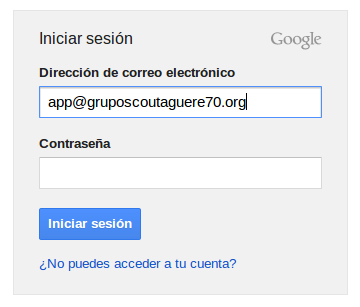
\includegraphics[width=0.5\textwidth]{images/login.jpg}
\caption{Ventana de login}
\label{fig:login}
\end{center}
\end{figure}


%++++++++++++++++++++++++++++++++++++++++++++++++++++++++++++++++++++++++++++++
\section{Gestión de socios}
\label{3:sec2}

Como se ha dicho a lo largo de la memoria, GScout esta enfocada a la gestión de socios, concretamente Scouts del grupo Aguere 70, 
por tanto la aplicación brinda la posibilidad de crear socios, visualizar sus datos, incluso podemos editarlos y/o borrarlos. Además existe una funcionalidad que nos permiten 
crear familias dentro de la aplicación, para asociar unos socios con otros, creando de esta manera un árbol de familia, el cual nos permite tener un contacto directo con los representantes de dichos
socios en caso de cualquier incidencia o necesidad. Por otro lado muchos de los socios podrían estar bajo medicación, de modo que la aplicación posee otra funcionalidad encargada de asociar medicación a los socios,
en la que se señalan las pautas y dosís que se deben de seguir con cada medicamento.\\

A continuación se detallará cada una de estas funciones que nos proporciona la aplicación GScout.\\

\subsection{Creación de Socios}

Los usuarios podrán crear nuevos socios rellenando los formularios predefinidos en la aplicación, dónde se clasifican los datos en personales, económicos, familiares y médicos.\\

En la Figura \ref{fig:form} se puede apreciar una parte de estos formularios para la creación de socios.

\begin{figure}[H]
\begin{center}
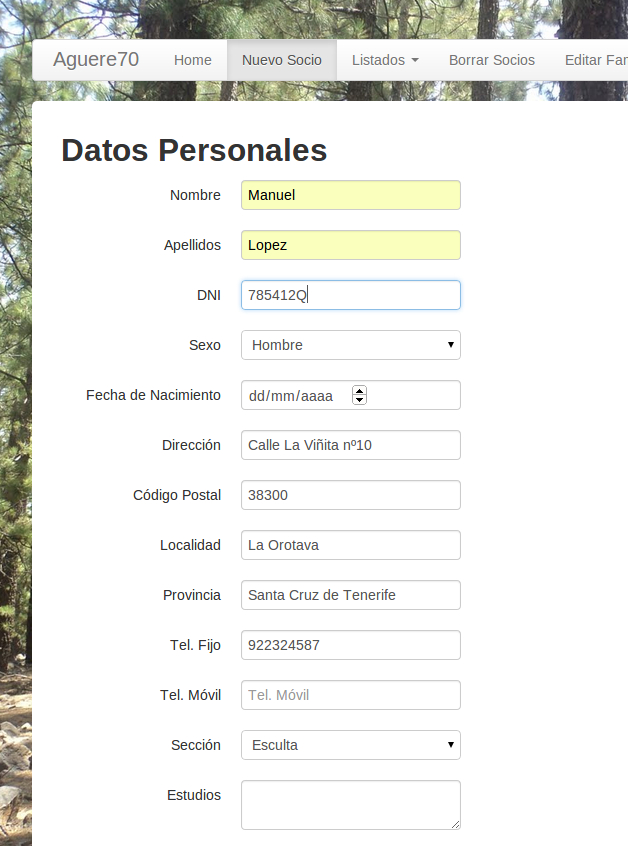
\includegraphics[width=0.5\textwidth]{images/ejemplo_formulario_personal.jpg}
\caption{Ejemplo de Formulario}
\label{fig:form}
\end{center}
\end{figure}

\subsection{Visualización y Edición de Socios}

Una vez creados los socios podremos visualizar su información accediendo a la ficha de socio, donde la informacion se divide en 4 pestañas: Personales, Familia, Economicos y Médicos \\

En la Figura \ref{fig:ficha_socio} se ve un claro ejemplo de como se visualizan los datos, en este caso los datos personales del socio.\\

\begin{figure}[H]
\begin{center}
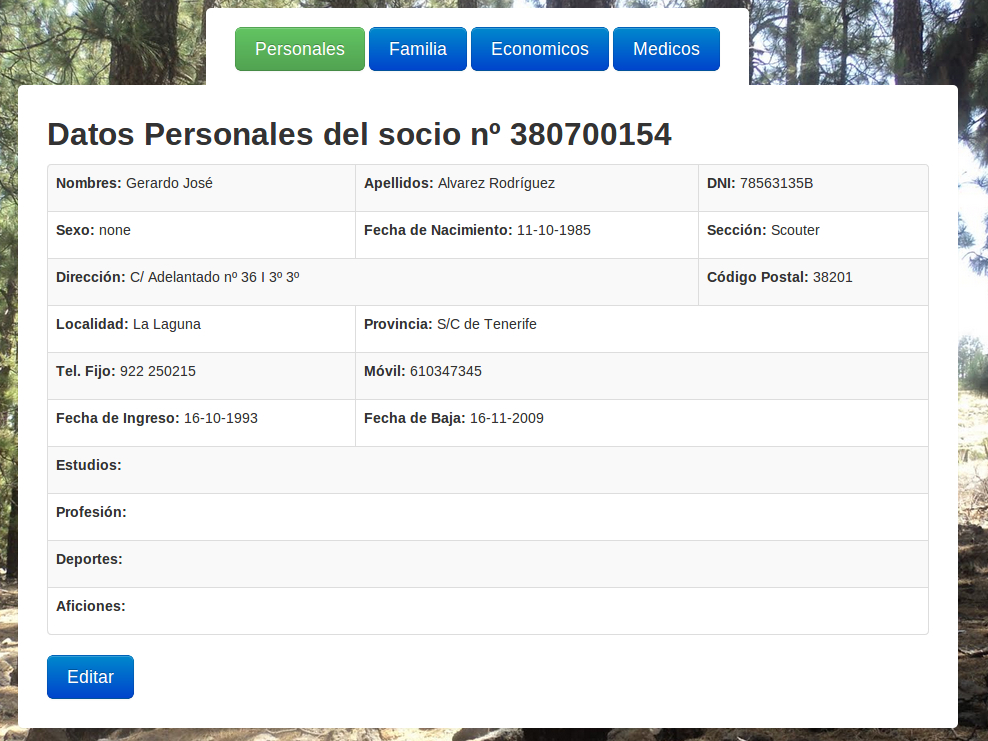
\includegraphics[width=0.75\textwidth]{images/datos_personales.jpg}
\caption{Ficha del Socio}
\label{fig:ficha_socio}
\end{center}
\end{figure}

Tambien se pueden editar sus datos, de una manera similar a la de creación de socios, simplemente buscamos el socio y le damos a editar (boton de la Figura \ref{fig:edit}), en la pestaña del tipo de información
que querramos cambiar.\\

\begin{figure}[H]
\begin{center}

\includegraphics[width=0.15\textwidth]{images/boton_editar.jpg}
\caption{Boton de Editar}
\label{fig:edit}
\end{center}
\end{figure}

\subsection{Borrado de Socios}
Tambien podremos borrar los socios, de momento los socios se borran permanentemente, pero en el modelo de datos esta configurado pera poder implementar un metodo que en vez de borrarlos los socios pasen
a un estado inactivo.\\

En la Figura \ref{fig:borrar_socio} se ve la pantalla dónde se seleccionan los socios que se desean borrar.\\

\begin{figure}[H]
\begin{center}
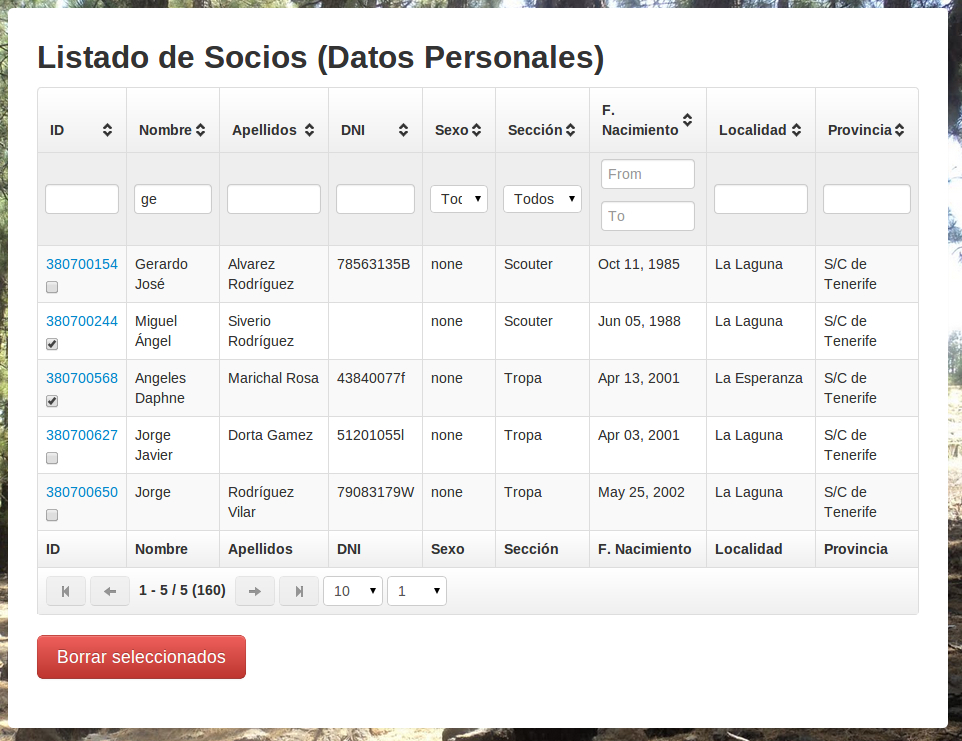
\includegraphics[width=0.75\textwidth]{images/borrado_socios.jpg}
\caption{Borrado de Socios}
\label{fig:borrar_socio}
\end{center}
\end{figure}

\subsection{Familiares}

Es obligado que cada socio pertenezca a una familia, la cual tendra un responsable que sera el indentificador de la familia, a la que se le pueden asignar varios socios, padres y/o tutores. En cierto modo, podremos
formar lo que seria un arbol de familia entre los socios, saber que socios conviven en la misma familia, saber quienes son los padres/tutores del socio, etc.\\

Un ejemplo de familia dentro de la aplicación lo podemos ver en la Figura \ref{fig:familia}.\\

\begin{figure}[H]
\begin{center}
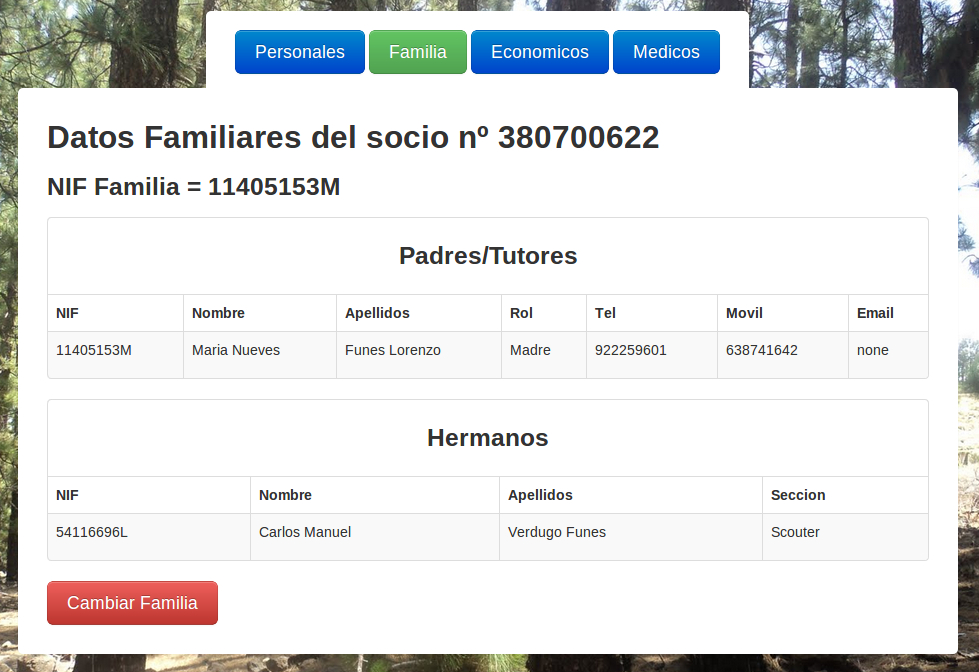
\includegraphics[width=0.75\textwidth]{images/familia_socio.jpg}
\caption{Ejemplo de Familia}
\label{fig:familia}
\end{center}
\end{figure}

Tambien GScout nos da la opción de cambiar o crear una familia nueva, por cualquier circunstancia que pueda pasar, en la que se necesite modificar las familias ya existentes.
Como muesta la Figura \ref{fig:edit_familia}.\\

\begin{figure}[H]
\begin{center}
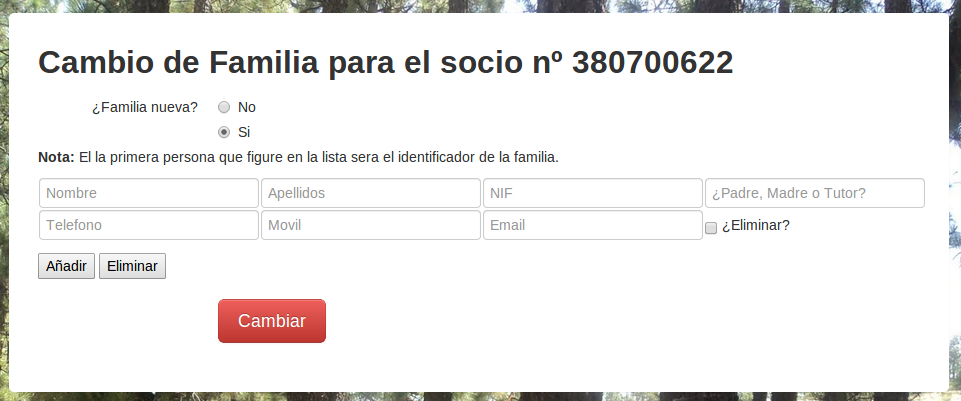
\includegraphics[width=0.75\textwidth]{images/cambio_familia.jpg}
\caption{Edición de Familia}
\label{fig:edit_familia}
\end{center}
\end{figure}


\subsection{Medicamentos}

Muchos de los socios podrían estar bajo medicación de algún tipo, por tanto existe un modulo en el que podemos anexar a los socios los datos de sus medicamentos, como el nombre, las pautas y las dosis correspondientes, 
como se muestra en la Figura \ref{fig:medicamentos}.\\

\begin{figure}[H]
\begin{center}
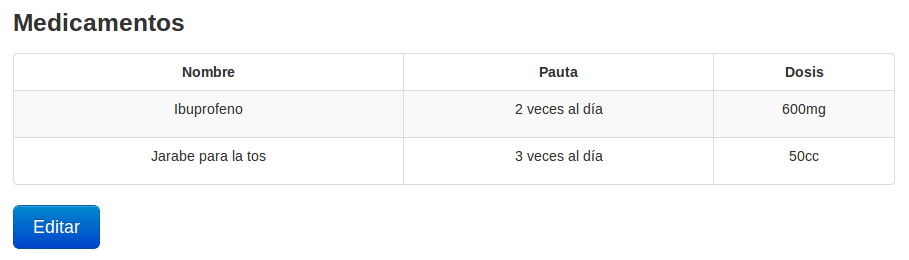
\includegraphics[width=0.75\textwidth]{images/medicamentos.jpg}
\caption{Medicamentos}
\label{fig:medicamentos}
\end{center}
\end{figure}

%++++++++++++++++++++++++++++++++++++++++++++++++++++++++++++++++++++++++++++++
\section{Cambios de unidad}
\label{3:sec3}

A petición de la organización scout Aguere 70 se creó una función que llamada \textbf{Cambio de Unidad} que consistes en analizar todos los socios, verificar su edad, y si procede cambiarlo a la sección/unidad acorde a su edad,
cuyo rango se muestra en la Figura \ref{fig:rango}.\\

\begin{figure}[H]
\begin{center}
\begin{tabular}{c|p{25mm}c|p{25mm}|} \hline 
\textbf{Intervalo(Años)} & \textbf{Unidad} \\ \hline
0-11 &
Manada
\\
\hline

11-14 &
Tropa
\\
\hline

14-17 &
Esculta
\\
\hline

17-20 &
Rover
\\
\hline

20+ & 
Scouter
\\
\hline
\end{tabular}
\caption{Rango de edades}
\label{fig:rango}
\end{center}
\end{figure}

Esta función se ejecuta al darle al botón de cambio de unidad que se encuentra en el menú principal (Figura \ref{fig:cambio_unidad}).\\


\begin{figure}[H]
\begin{center}

\includegraphics[width=0.40\textwidth]{images/cambio_unidad.jpg}
\caption{Botón Cambio de Unidad}
\label{fig:cambio_unidad}
\end{center}
\end{figure}

%++++++++++++++++++++++++++++++++++++++++++++++++++++++++++++++++++++++++++++++
\section{Listados de información}
\label{3:sec4}

Hay una sección en la aplicación en la que podemos listar los socios visualizando sus datos dependiendo del listado, es decir, existen un listado especifico para los datos personales y otro para los datos economicos.\\

En estos listados podremos interactuar filtrando los datos por medio de varios filtro, incluso ordenarlos alfabeticamente en orden creciente y decreciente si se desea.\\

En la Figura \ref{fig:listado} se muestra un ejemplo de una pantalla de listado.

\begin{figure}[H]
\begin{center}
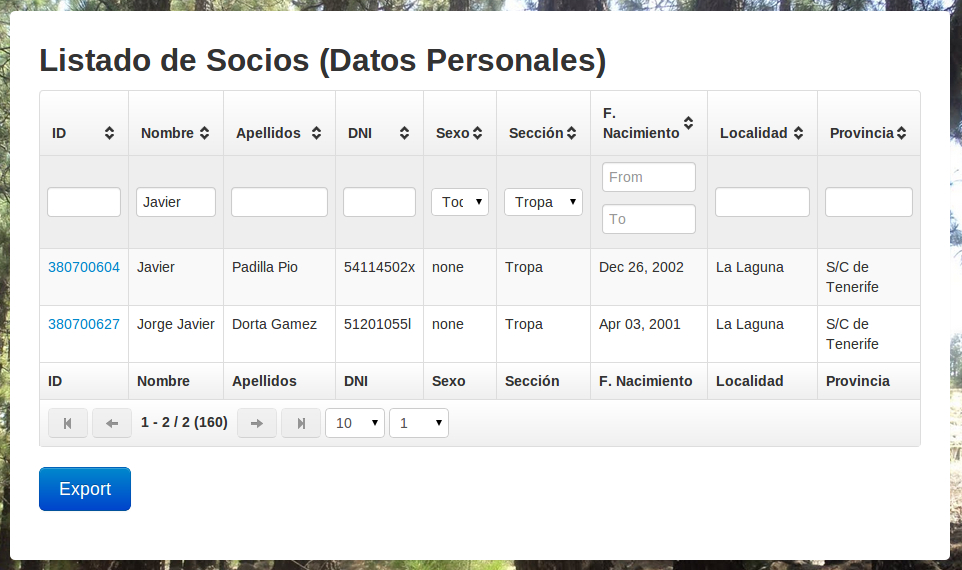
\includegraphics[width=0.75\textwidth]{images/filtrado.jpg}
\caption{Aplicación de algunos filtros al listado}
\label{fig:listado}
\end{center}
\end{figure}


%++++++++++++++++++++++++++++++++++++++++++++++++++++++++++++++++++++++++++++++
\section{Busquedas por ID}
\label{3:sec5}

Tambien se pueden realizar busquedas directas por el ID del socio, como se muestra en la Figura \ref{fig:busqueda_id}, en la que nos redirecciona a directamente  a la ficha técnica del socio.\\

\begin{figure}[H]
\begin{center}
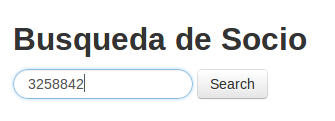
\includegraphics[width=0.40\textwidth]{images/busqueda_id.jpg}
\caption{Busqueda ID}
\label{fig:busqueda_id}
\end{center}
\end{figure}

%++++++++++++++++++++++++++++++++++++++++++++++++++++++++++++++++++++++++++++++
\section{Exportaciones}
\label{3:sec6}

Los resultados de los listados los podemos exportar a Google Drive en formato de hoja de calculo, con solo darle al botón de exportar debajo del listado. Veamos un ejemplo con imagenes:\\

En la Figura \ref{fig:list_export} se muestra el listado que se desea exportar.
\begin{figure}[H]
\begin{center}
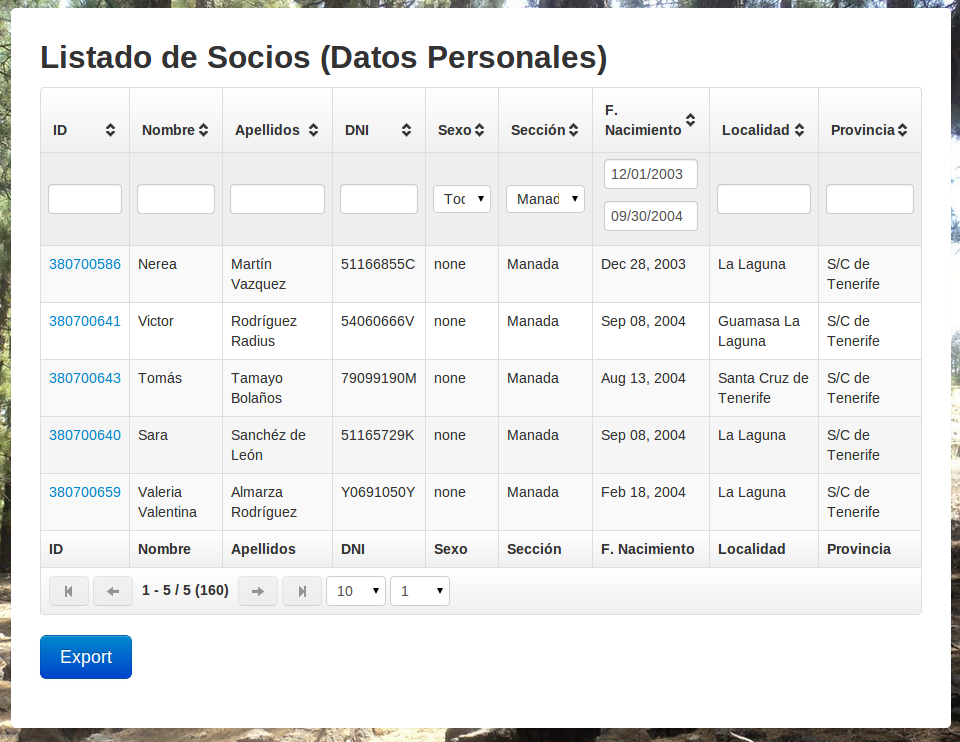
\includegraphics[width=0.75\textwidth]{images/listado_export.jpg}
\caption{Exportación de un listado}
\label{fig:list_export}
\end{center}
\end{figure}

Al darle al botón exportar, se crea un documento en la cuenta de Drive del usuario con los datos que se exportaron, como se muestra en la Figura \ref{fig:export_drive}.\\

\begin{figure}[H]
\begin{center}
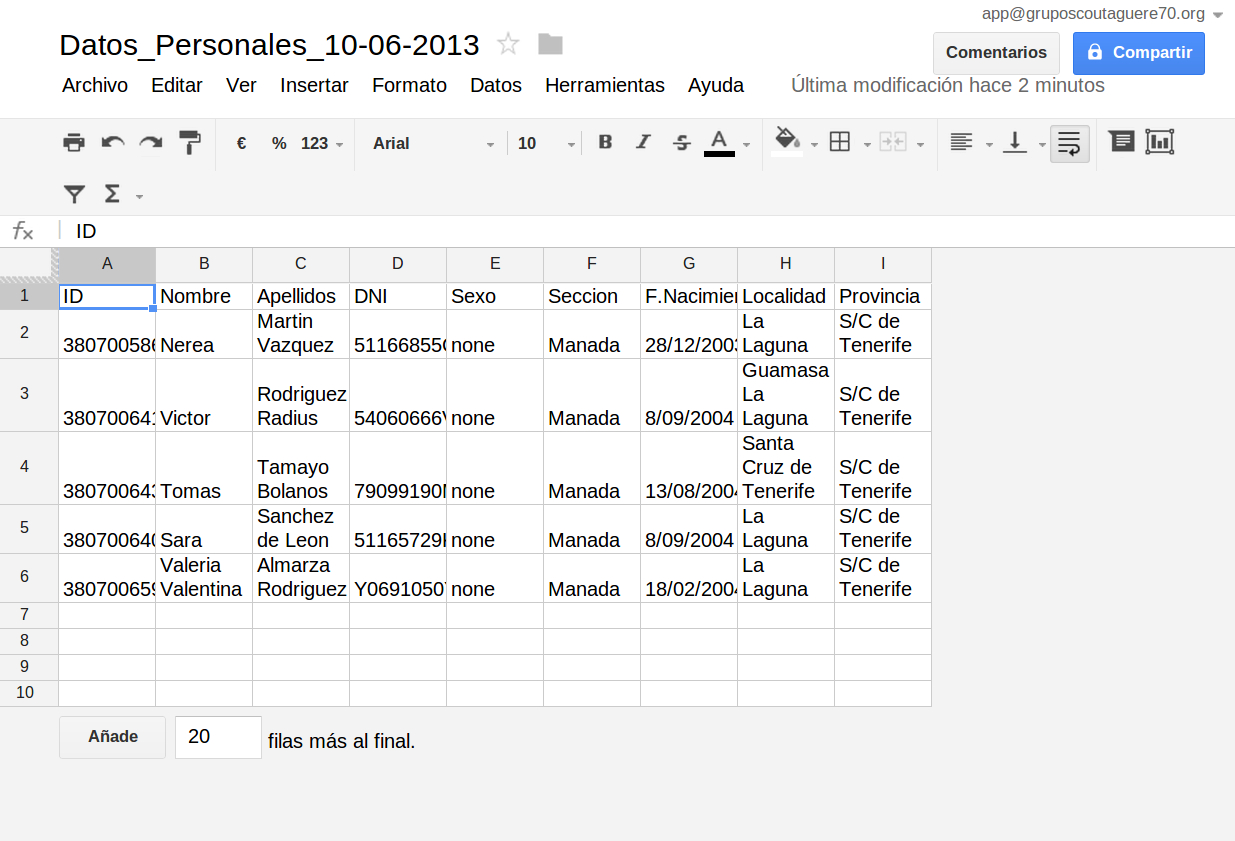
\includegraphics[width=0.75\textwidth]{images/result_export.jpg}
\caption{Resultado de la Esportación}
\label{fig:export_drive}
\end{center}
\end{figure}

%++++++++++++++++++++++++++++++++++++++++++++++++++++++++++++++++++++++++++++++
\section{Importaciones}
\label{3:sec7}

GScout brinda a la organización de scout Aguere 70 la posibilidad de migrar su base de datos en \textbf{Access} a la propia aplicación, siempre y cuando este fichero se transforme en un archivo .csv, con la herramienta MDB Tools por ejemplo,
y solo haría falta subirla a la aplicación, lo demás lo hace la propia aplicación de manera automática. De esta manera tendremos los datos de la antigua base de datos en la nueva base de datos que pertenece a GScout.\\

En la Figura \ref{fig:import} se ve un ejemplo del proceso de importación.\\ 
\begin{figure}[H]
\begin{center}
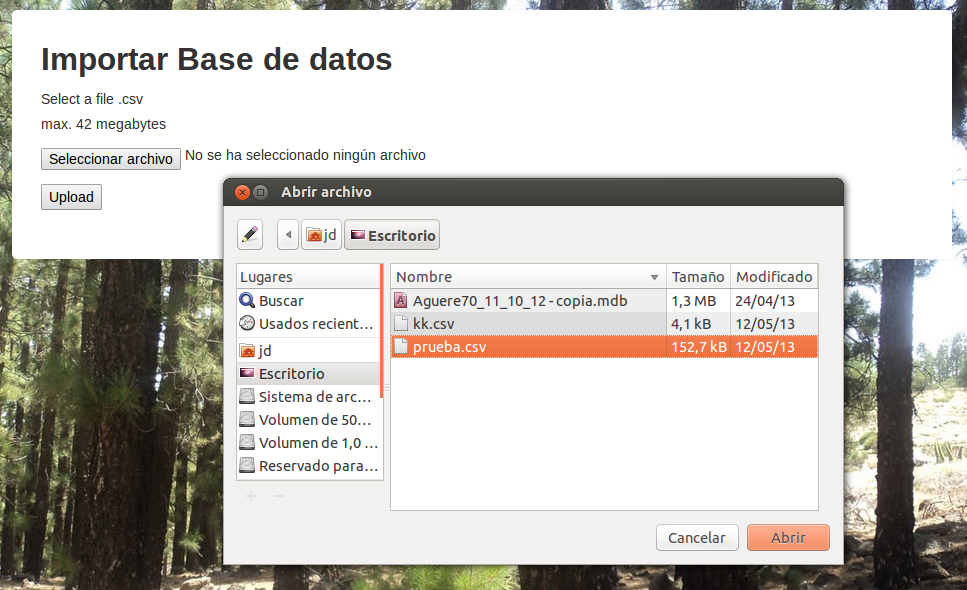
\includegraphics[width=0.75\textwidth]{images/import_db.jpg}
\caption{Subiendo archivo csv para importar base de datos}
\label{fig:import}
\end{center}
\end{figure}

Esta función se ejecuta al darle al botón de la Figura \ref{fig:import} que se encuentra en el menú principal.\\


\begin{figure}[H]
\begin{center}

\includegraphics[width=0.40\textwidth]{images/import.jpg}
\caption{Botón Importar Base de Datos}
\label{fig:import}
\end{center}
\end{figure}